\documentclass[11pt]{article}
\usepackage[margin=1in]{geometry}
\usepackage[T1]{fontenc}
\usepackage{lmodern,amsmath,amssymb,amsthm,graphicx,booktabs,array}
\input{ot1lmr.fd}
\DeclareFontShape{T1}{lmr}{m}{n}{<-> ec-lmr10}{}
\DeclareFontShape{OT1}{lmr}{m}{n}{<-> rm-lmr10}{}
\input{omllmm.fd}
\DeclareFontShape{OML}{lmm}{m}{it}{<-8.5> lmmi8 <8.5-> lmmi10}{}
\usepackage{enumitem,microtype,caption,fancyhdr}
\usepackage[colorlinks=true,linkcolor=black,citecolor=black,urlcolor=blue]{hyperref}
\setlength{\emergencystretch}{2em}
\setlength{\parskip}{0.2em}
\setlength{\headheight}{14pt}
\captionsetup{font=small,labelfont=bf}
\pagestyle{fancy}\fancyhf{}
\fancyhead[L]{\small Shaping Gap Benchmark II}
\fancyfoot[C]{\thepage}
\newtheorem{proposition}{Proposition}
\newcommand{\R}{\mathbb{R}}
\newcommand{\silu}{\operatorname{SiLU}}
\newcommand{\rms}{\operatorname{rms}}
\newcommand{\eps}{\varepsilon}
\makeatletter\let\rawinput\@@input\makeatother
\hypersetup{pdftitle={Shaping Gap Benchmark II: Scalable Effect-Interface Evaluation and Verified Functional Construction},pdfauthor={Nathaniel Oh and Paul Attie}}
\title{Shaping Gap Benchmark II:\\Scalable Effect-Interface Evaluation\\and Verified Functional Construction}
\author{Nathaniel Oh \and Paul Attie}
\date{November 12, 2026}
\begin{document}
\maketitle
\thispagestyle{plain}
\begin{abstract}
An acquired description of frozen neural computation is useful only if a runtime
can afford to compose it and can turn it into executable behavior. We extend
Shaping Gap Benchmark in both directions. First, a response-moment evaluator
computes predecessor-conditioned pair effects without materializing candidate
pair states. Its retained arrays scale as $O(Kn+K^2+Mn)$ and tiled forecast
workspace as $O(tKm+K)$ for $K$ components, state width $n$, $M$ retained readouts,
$m$ required coordinates and tile size $t$. On five nested banks from 22 to 512
original frozen SwiGLU components, the method preserves direct forecast rankings
and remains inside a 64 MiB controller-array envelope. At 128 components it
satisfies all 72 numerical contracts, versus 58 for native local guidance,
with 57.50\% less native projection-equivalent work after source acquisition,
deployment and independent selected-program verification. Second, the same
sealed 512-component bank constructs a fixed program for each externally
specified Boolean function, jointly over all inputs. Across eight functions
and three numeric encodings, both one-step and paired guidance implement all
24 truth tables exactly. Paired guidance meets a stricter output margin on
23 targets versus 22 and uses 26.00\% less charged native work, while taking
more search time. All 768 selected programs replay bit exactly through original
native components; weights remain unchanged. The contribution is a scalable
evaluator for acquired effect interfaces and a verified finite-function
construction result, establishing an executable starting point for subsequent
capability-interface acquisition and reuse.
\end{abstract}

\section{Introduction}
A frozen pretrained model contains computations that can be executed outside
their original whole-model schedule. The first Shaping Gap Benchmark paper
introduced effect interfaces: reusable descriptions of how native components
change monitored state and how predecessor context changes their response
\cite{sgb1}. A runtime uses those descriptions to construct temporary programs
satisfying explicit requirements. That study established the interface and its
construction value over 22 components, three local domains and 288 contracts.

Two subsequent questions determine whether that foundation can support a larger
research program. Can the runtime reason over a substantially larger repertoire
without a prohibitive forecast workspace? Can construction produce a fixed
function over multiple inputs, rather than satisfy a numerical requirement at
one particular activation? These questions concern the same computational
material: retained descriptions support selection and composition, while original
frozen components determine the executed answer.

We address the first question by factoring pair responses into reusable response
moments. Instead of constructing every $x_{AB}$ and projecting it again, the
runtime combines scalar activities with precomputed cross-component responses.
This removes the need for a pair-by-state-width tensor. Scoring is specialized
to the requirement's coordinates and streamed in tiles. Preparation, retained
arrays, online work and native checks are all measured.

For the second question, we adopt the specification-and-grammar perspective of
syntax-guided synthesis \cite{sygus,standard}. A target truth table defines
success independently of the neural response interface. The grammar contains
original native components. One fixed sequence must implement the function on
every input, with activities recomputed from live state; the runtime cannot choose
a different program for each row. Numeric input and output conventions are fixed
independently of the requested function.

The resulting contribution has three parts:
\begin{enumerate}[leftmargin=*,itemsep=0.15em]
\item A response-moment evaluator with explicit algebraic and resource bounds,
      validated against direct pair-state evaluation.
\item A controlled 22-to-512-component construction study, with common contracts,
      source-inclusive costs and independent native verification.
\item An exhaustive finite-function construction study using the same sealed bank,
      with one program per target, a one-step interface control, output-margin
      checks and a complete native-work ledger.
\end{enumerate}

The scope is deliberately executable: these studies concern one frozen checkpoint,
supplied architectural form and finite component banks. Their role in the broader
program is to make functional constructions available as future objects of
interface acquisition, retention and reuse. Repeated acquisition of higher-level
interfaces is a subsequent experiment, rather than a property assumed here.

\section{Computational setting and effect interfaces}
\label{sec:setting}
Let $x\in\R^n$ be live activation. A component $b$ is one original SwiGLU neuron,
including its original down-projection direction:
\begin{align}
 F_b(x)&=x+d_b a_b(x), &
 a_b(x)&=\silu\!\left(\frac{g_bx}{r(x)}\right)
                    \frac{u_bx}{r(x)},\label{eq:atom}\\
 r(x)^2&=x^Tx/n+\eps, & q(x)&=Qx/r(x).\label{eq:readout}
\end{align}
Normalization weights are absorbed into the rows $g_b,u_b,Q$. A program is a
sequence $p=(b_1,\ldots,b_\ell)$, with $F_p=F_{b_\ell}\circ\cdots\circ F_{b_1}$.
There are no trainable amplitudes or fitted output heads. Each component's live
activity determines its write. Source directions, encoders, readout coordinates
and component boundaries are supplied or acquired as described below.

The accumulated effect and its incoming-context partial are
\begin{equation}
 E_b(x)=q(F_b(x))-q(x),\qquad K_b(x)=D_xE_b(x).
\end{equation}
For a predecessor displacement $v$, the change in successor effect is
\begin{equation}
 E_b(x+v)-E_b(x)=\int_0^1K_b(x+tv)v\,dt.
\end{equation}
This identity from the first paper motivates a compatibility forecast rather
than treating components as fixed additive effects. Here we use its
\emph{structure-calibrated} representation: the RMS/SwiGLU law is supplied,
and numerical coefficient rows are recovered from original native observations
and partials. We do not fit a new semantic law or claim architectural discovery.

For a normalized linear scalar $y(x)=wx/r(x)$, the coefficient row is recoverable
at a calibration anchor as
\begin{equation}
 w=r(x)D_xy(x)+\frac{y(x)x^T}{nr(x)}.\label{eq:calibration}
\end{equation}
This follows by differentiating $wx/r(x)$ and rearranging. The original native
direction $d_b$ is acquired using a unit hidden activation through its original
down projection. These identities are statements in real arithmetic under the
supplied form. Quantized native projection and float32 rounding remain subject
to independent checks; a calibrated surrogate is not substituted for the native
execution authority.

\section{Response-moment composition}
Let $D=[d_1\ \cdots\ d_K]$, and stack the acquired rows in $G,U$. Retain
\begin{equation}
 GD,\quad UD,\quad H=D^TD,\quad QD
\end{equation}
along with $G,U,D,Q$ and the physical coordinate operator $P=(D^TD)^{-1}D^T$
for the full-rank banks considered here. The preparation cost includes forming
these products and solving for $P$.

\begin{proposition}[Pair response from retained moments]
Under Equations~\eqref{eq:atom}--\eqref{eq:readout}, let $t=a_A(x)$ and define
\begin{align}
 s_A&=\frac{x^Tx+2t x^Td_A+t^2H_{AA}}{n},\\
 v_B&=\silu\!\left(\frac{g_Bx+t(GD)_{BA}}{\sqrt{s_A+\eps}}\right)
             \frac{u_Bx+t(UD)_{BA}}{\sqrt{s_A+\eps}},\\
 s_{AB}&=s_A+\frac{2v_B(x^Td_B+tH_{AB})+v_B^2H_{BB}}{n}.
\end{align}
Then the pair readout is
\begin{equation}
 q(F_B(F_A(x)))=
 \frac{Qx+t(QD)_A+v_B(QD)_B}{\sqrt{s_{AB}+\eps}}.\label{eq:pair}
\end{equation}
\end{proposition}
\begin{proof}
Substitute $x_A=x+td_A$ into the linear gate and up numerators, giving
$g_Bx_A=g_Bx+t(GD)_{BA}$ and its up counterpart. Expanding
$\|x_A\|^2$ yields $s_A$. Expanding $\|x_A+v_Bd_B\|^2$ yields $s_{AB}$.
The linear readout numerator is $Qx+tQd_A+v_BQd_B$; dividing by the final
RMS factor gives Equation~\eqref{eq:pair}.
\end{proof}

\paragraph{Tiling and contract specialization.}
Only the $m$ required readout coordinates enter a forecast score. We sweep first
components $A$ in tiles of $t$ rows, compute their $K$ continuations and retain
one best continuation score per first component. The stopping option competes
with taking a successor. At the terminal search depth, only the one-step option
is scored. Native observation at the current state centers the readout forecast
to reduce numerical offset from acquired coefficients.

Retained arrays cost $O(Kn+K^2+Mn)$, where $M$ counts all retained readout rows.
Forecast temporaries cost $O(tKm+K)$, in addition to search-state arrays.
No $K\times K\times n$ pair-state tensor or $K^3$ latent-coordinate tensor is
required. Evaluating all pairs still entails quadratic work in $K$; forming
moments also has a nonzero preparation cost. These bounds describe the explicit
representation, not total process memory or unlimited scaling at fixed memory.

\paragraph{Construction.}
The controller ranks first components by their best legal one- or two-step
continuation. A beam expands up to six children per parent, then executes each
proposed first component through original native projections. It evaluates the
actual result, retains the best states and repeats. Pair predictions guide
which first steps to try; they do not replace native branch evaluation. Activity
caching across siblings is charged and separately bounded.

\section{Experimental design and accounting}
\subsection{Common substrate and provenance}
Both studies use \texttt{Qwen/Qwen3-0.6B-MLX-4bit}, at revision\\
\texttt{173234aa840d113125e9f2271100ddbaf16c9620}, with MLX 0.32.4,
MLX-LM 0.32.2 and NumPy 2.5.4 on an Apple M4 Max with 36 GiB memory.
The stored parameter arrays occupy 316,747,776 bytes. The full loaded-parameter
digest is recorded in the artifact and checked before and after execution.
The original model forward, transformer-block forward, attention, embeddings
and token output paths are guarded against execution. The checkpoint supplies
original parameter-backed fragments; no hosted inference, language prompting,
tokenization, adapter training or pretrained-weight updates occur.

The initial 22 components are inherited from the first study, and their
historical discovery is charged. A seeded uniform permutation of original
neuron identifiers appends distinct components to reach 512. Nested prefixes
give bank sizes 22, 64, 128, 256 and 512. Responses are calibrated at one fixed
anchor before later outcomes are exposed. Directions and the source bank are
sealed; the second study uses that bank without refitting. Selection of the
additional units does not inspect later targets.

\subsection{Numerical construction: P48}
The registered scaling study fixes 72 common contracts: four upward demands
$0.025$, $0.05$, $0.075$ and $0.1$, three domains and six roots per domain/demand.
Roots are perturbed only in the original 22-direction span, so they are identical
across bank sizes. Each contract selects six of twelve domain readouts: three
targets must increase by the demand, while three protected coordinates remain
within $0.05$ of their initial values. Contract satisfaction uses tolerance
$10^{-5}$.

Native-local sensitivity guidance is compared with acquired paired guidance.
The native-local controller queries current native readouts/partials and uses
local displacement scores; the treatment acquires behavioral rows in advance
and forecasts conditioned continuations. Both access the same native component
bank and checker, with a maximum of 512 LPE per search, beam width four, six
children and depth six. Their different source access and acquisition costs are
explicit rather than treated as equal information at no cost.

Every component must have absolute amplitude at most 2, write RMS at most 0.15,
live-state RMS at most 2 and bounded physical coordinates within radius 1.5.
The explicit controller-array envelope is 64 MiB, including an 8 MiB reservation
for search arrays. The native activity cache has its own 1 MiB limit. Full
process and MLX peaks are measured separately.

The evaluator diagnostic compares direct activation-space pair construction
with response moments on three fixed contexts per bank. It checks predicted
readouts, successor activities and the first six ranked choices. The two
implementations use identical calibrated coefficients. Direct evaluation uses
two-row tiles and response moments sixteen-row tiles, each within its declared
array envelope; this compares feasible implementations, not tile-matched kernels.

\subsection{External finite functions: P49}
Eight Boolean functions are fixed before execution: two-input AND, OR and XOR;
three-input AND, OR, XOR, majority and multiplexer. For multiplexer,
$f(b_0,b_1,b_2)=b_1$ if $b_0=1$, otherwise $b_2$. Three encoder seeds give 24
function/encoding targets. The finite input domains have four or eight rows.

Let $q_0$ be one fixed native readout. A random frame and three orthogonal bit
directions are projected into its acquired linear numerator's nullspace. Their
RMS magnitudes are 0.25 and 0.1, respectively. Bits are encoded as signed
displacements along those directions; decoding is the sign of $q_0$.
The frame, directions and decoder do not depend on the target function. This
supplied numeric I/O convention creates a controlled construction assay; it is
not a natural text-input distribution.

For target $f$, the same sequence $p$ must satisfy
\begin{equation}
 \mathbf{1}[q_0(F_p(\operatorname{enc}(b)))>0]=f(b)
 \quad\text{for every }b\in\{0,1\}^w.\label{eq:bool}
\end{equation}
The stricter outcome requires signed output at least 0.025, allowing numerical
tolerance $10^{-5}$. Search minimizes the sum of squared margin deficits across
\emph{all} inputs jointly. It sees the full finite specification. This is
finite-domain synthesis, not held-out-input learning.

One-step and paired acquired-interface guidance share the same bank, joint
program grammar, checker, physical constraints, beam and child limits. Each
search permits 32,768 native LPE and depth 16. Method order alternates by target.
No hand-assigned logical role or answer program is supplied to a component.

\subsection{Cost scopes}
\label{sec:cost}
LPE counts native linear projections and recorded transpose-projection queries.
Normalization and scalar planning are recorded but not assigned projection
units; LPE is not FLOPs, joules or equal hardware cost per operation. Our main
charged-work tables include historical inventory discovery, inherited domain
setup, source acquisition, all attempted native branch work, initial readouts,
one deployment and independent selected-program verification. The inherited
inventory is 3,199 LPE and domain setup 3 LPE. A $K$-unit treatment pays $K$
direction queries and $4K+75$ behavioral calibration LPE; the native-local arm
does not pay for unused behavioral calibration. Each functional arm is charged
the entire 512-unit source again for its standalone comparison.

Storage remains a byte measurement. Preparation and scalar planning have
separate time measurements. The arrays are unchanged throughout both studies,
so there are no refitting, eviction or maintenance events. Source diagnostic
validation, microbenchmark probes and additional sampled-branch auditing are
separately recorded with complete primitive vectors. They are not hidden in the
selected-program verification count. All failed construction attempts remain
in the trace. Complete experiment wall, measured algorithm components and
independent-verifier wall are distinguished; shared startup and unallocated
driver overhead are not assigned to either method.

\section{Results}
\subsection{A larger bank improves the finite construction frontier}
Table~\ref{tab:scaling} and Figure~\ref{fig:scaling} show all banks and both
methods. Paired guidance reaches 72/72 contracts at 128 components, compared
with 58/72 for native-local guidance. Charged native work is 11,691 versus
27,510 LPE, a 57.50\% reduction. The 128-unit treatment also exceeds the
512-unit baseline's solve count, 72 versus 70, with 27.63\% less charged work.
Both methods benefit from the larger repertoire. The comparison therefore
measures construction value over common material, rather than assigning every
bank-size improvement to the interface.

\begin{table}[t]
\centering\small
\begin{tabular}{r rr rr}
\toprule
&\multicolumn{2}{c}{Satisfied / 72}&\multicolumn{2}{c}{Charged native LPE}\\
Components&Native local&Paired&Native local&Paired\\\midrule
22&17&36&35,946&28,767\\
64&39&67&30,719&16,735\\
128&58&72&27,510&11,691\\
256&69&72&21,216&9,055\\
512&70&72&16,154&8,649\\\bottomrule
\end{tabular}
\caption{Common contracts, matched 512-LPE online allowance. Charged work
includes acquisition, construction, deployment and independent selected-program
verification; additional research diagnostics are separately recorded.}
\label{tab:scaling}
\end{table}

\begin{figure}[t]
\centering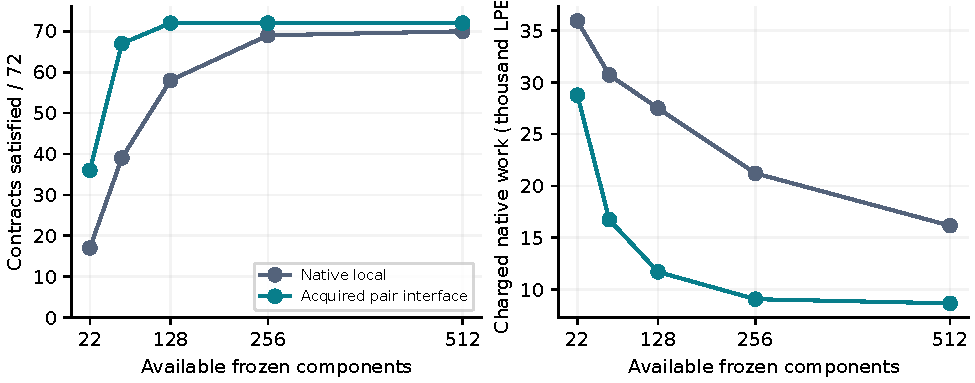
\includegraphics[width=\linewidth]{figures/scaling.pdf}
\caption{Finite construction frontier and charged native work as the bank grows.
Each point uses the same 72 contracts. The bank-size axis increases the repertoire;
program depth remains capped at six.}
\label{fig:scaling}
\end{figure}

All fifteen direct/factored evaluator comparisons preserve the first six ranked
choices. The maximum absolute discrepancy across readouts and activities is
$1.14\times10^{-12}$. Source validation over twelve native states gives maximum
readout error $1.44\times10^{-6}$ and amplitude error $5.61\times10^{-5}$.
These are finite diagnostics, not uniform error certificates over arbitrary
states.

At 512 units, retained bank arrays occupy 23,527,424 bytes and the conservative
controller-array reservation is 40,435,712 bytes, below 64 MiB
(Figure~\ref{fig:resources}). Full process peak is 613,302,272 bytes, including
the checkpoint; MLX peak is 317,472,848 bytes. The controller reservation excludes
the checkpoint and runtime overhead, which remain in process memory.

\begin{figure}[t]
\centering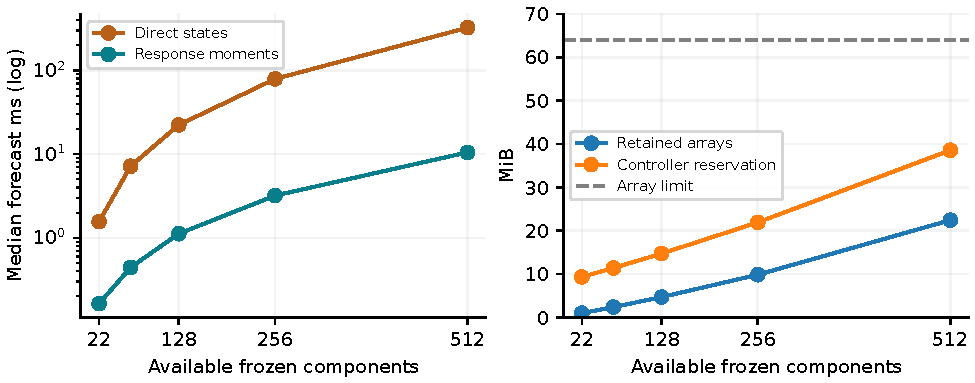
\includegraphics[width=\linewidth]{figures/resources.pdf}
\caption{Exploratory evaluator timing and explicit array measurements. Timing
uses three contexts per bank, fixed direct-then-factored order and different
feasible tile sizes. Whole-process peak is 585 MiB; the 64 MiB line is the
controller-array envelope.}
\label{fig:resources}
\end{figure}

The median 512-unit evaluator diagnostic takes 324.2 ms with direct states and
10.5 ms with response moments. This fixed-order, three-context timing is
exploratory. Measured source/preparation/search/deployment components at 128
units total 3.78 s native-local and 1.95 s paired. At 512 units, paired is slower:
2.58 s versus 2.35 s, despite its native-work advantage. Complete P48 run wall is
36.56 s and independent replay 2.48 s. These measurements support a native-query
and workspace gain, with a bank-dependent time tradeoff.

\subsection{A fixed program implements each finite function}
Both methods satisfy Equation~\eqref{eq:bool} on all 24 function/encoding targets.
Each selected graph is used unchanged across its entire four- or eight-input
domain. The empty program meets the robust criterion on none of the 24 targets.
Paired guidance meets the stricter output margin on 23 targets, versus 22 for
one-step guidance (Tables~\ref{tab:functions}--\ref{tab:byfunction}).

\begin{table}[t]
\centering\small
\begin{tabular}{lrr}
\toprule
Outcome&One-step&Paired\\\midrule
Exact truth tables&24/24&24/24\\
All outputs meet margin&22/24&23/24\\
Construction native LPE&35,460&24,436\\
Source + construction + deployment LPE&43,325&31,917\\
With independent selected verification&45,353&33,561\\
Aggregate search time (s)&7.31&11.94\\
Median selected program length&2&2\\\bottomrule
\end{tabular}
\caption{Functional construction at matched exact Boolean quality. Both arms
use acquired structured interfaces; paired guidance improves native-work and
margin outcomes, while taking more search time.}
\label{tab:functions}
\end{table}

The charged-work reduction at matched exact Boolean quality is 26.00\%, including
independent selected-program verification. Construction alone uses 31.09\% fewer
native LPE. Paired aggregate search takes 11.94 s versus 7.31 s: the additional
forecast computation is not a free resource. Complete run wall is 21.43 s,
process peak 561,086,464 bytes, MLX peak 317,423,724 bytes and maximum controller
array reservation 58,130,432 bytes. Native verification adds 0.81 s.

\begin{table}[t]
\centering\small
\begin{tabular}{l rr rr rr}
\toprule
&\multicolumn{2}{c}{Exact / 3}&\multicolumn{2}{c}{Margin / 3}&\multicolumn{2}{c}{Construction LPE}\\
Function&One&Pair&One&Pair&One&Pair\\\midrule
\rawinput function-rows.tex
\bottomrule
\end{tabular}
\caption{Every specified function over all three encoders. LPE includes all
attempted native branch/input executions and initial readouts. XOR3 accounts
for the margin failures and much of the construction work.}
\label{tab:byfunction}
\end{table}

The paired margin failure is XOR3 under encoder 79001: signs are correct but
the minimum signed output is 0.021295. One-step also misses the margin on XOR3
under encoder 79003, with minimum signed output 0.023240. No failing target is
removed. Both exact and margin outcomes are reported because exact signs alone
would conceal the registered quality shortfalls.

\paragraph{A concrete constructed function.}
For XOR3 with encoder 79003, paired guidance selects the six-component sequence
with bank identifiers $(87, 98, 159, 372, 341, 190)$. Each identifier resolves to
an original layer/neuron pair in the artifact. The same six instructions run
on all eight inputs. Table~\ref{tab:example} gives native decoder values and the
independent parity specification. The one-step program has length 16 and gets
the signs right, but falls short of the required margin on one input. This
illustration was chosen after the registered study to expose the quality
difference; it is not an additional trial.

\begin{table}[t]
\centering\small
\begin{tabular}{rrrrrr}
\toprule
$b_0$&$b_1$&$b_2$&XOR&One-step $q_0$&Paired $q_0$\\\midrule
\rawinput example-rows.tex
\bottomrule
\end{tabular}
\caption{Complete native truth table for one constructed XOR3 function.
The decoding rule is $q_0>0$; the robust criterion additionally requires
absolute signed output at least 0.025, up to $10^{-5}$ numerical tolerance.}
\label{tab:example}
\end{table}

\subsection{Independent execution and portable replay}
The scaling verifier executes all 720 selected graphs through original native
masked-hidden projections and independently samples 512 of 21,591 recorded
branches. The function verifier checks all 48 graphs on all 312 input executions,
reconstructs each Boolean specification independently, checks the common encoders
and every intermediate physical limit, and verifies final states and readouts.
All selected graphs replay bit exactly. Complete primitive vectors match the
recorded ledgers; pretrained and acquired-source hashes are unchanged.

A separate NumPy-only replay executes all 768 selected programs from the
acquired structured bank, with no checkpoint or MLX import. All numerical
contract and function-margin decisions agree with native outcomes; all Boolean
decisions agree as well. Maximum readout error is $3.21\times10^{-5}$ over this
finite replay. This additional artifact check does not change the native trial
count or establish compression of the full model.

\section{Related work and interpretation}
The first Shaping Gap Benchmark paper \cite{sgb1} establishes the accumulated-effect
interface, incoming-context sensitivity and temporary native program runtime.
This paper extends its structure-calibrated reference with response-moment
evaluation and external finite-function specifications. It uses a different,
smaller common numerical contract set; its solve rates should not be compared
directly with the first paper's 288-contract rates.

Syntax-guided synthesis \cite{sygus,standard} supplies the separation between a
correctness specification and an implementation grammar. Here the grammar's
instructions are original frozen neural components, and their effects depend on
live state. Our Boolean suite is custom and finite; we report neither a SyGuS
competition result nor a performance comparison with symbolic synthesizers.
The contribution is the neural-component implementation path and its measured
construction cost. Exhaustive finite checking is the correctness method, not
a new verification algorithm.

Program-library learning, including DreamCoder \cite{dreamcoder}, demonstrates
how solved programs can supply reusable abstractions for later tasks. That is
a relevant building block for the next stage: acquire interfaces to the programs
constructed here, and measure whether they improve later acquisition after
retention and maintenance. This paper keeps the acquired component bank fixed
and does not claim to have executed that continuing library-growth loop.

Fixed nonlinear features can support useful functions without task-specific
changes to every feature parameter; random-feature methods provide a classical
example \cite{randomfeatures}. Our experiments execute original pretrained
components and do not fit a task-specific output head, but they do not compare
with matched random-weight substrates. Thus successful construction establishes
usability of this pretrained substrate, while the contribution attributable
specifically to pretraining remains an experimental question.

\section{Limits and next experiments}
The evidence spans one checkpoint, five nested finite banks, three numeric
domains and eight Boolean functions under three encoders. The encoder seeds
are not independent models, and the hundreds of program rows are not independent
pretraining trials. We report the full finite design rather than treating its
rows as population-level statistical replication.

The architectural law, readout rows and numeric I/O convention are supplied.
The Boolean inputs are exhaustive and available during construction. Larger
application impact requires more demanding independent specifications,
comparisons with established symbolic constructors and additional architectures.
Native-work savings need to be considered alongside forecast CPU time, process
memory and, in future, measured energy. A 64 MiB explicit-array envelope is not
a 64 MiB model or device footprint.

The next mechanism experiment is to acquire a reusable executable interface
to a successful constructed program and use it when constructing a later
compositional Boolean or bit-vector function. An informative comparison must
match specification access and final quality, charge first and subsequent
interface acquisition, and include regression checks, retention and maintenance.
That experiment would test whether construction knowledge compounds. The present
results provide the necessary concrete starting point: scalable component
forecasts and native programs with externally specified functional behavior.

\section{Conclusion}
Acquired effect interfaces can support a larger frozen-component repertoire
without materializing all pair states. In the measured study, response-moment
composition improves the finite construction frontier and lowers charged native
work. The same sealed bank also supports fixed programs implementing complete
Boolean functions. These results connect the first paper's interface/runtime
foundation to independently checkable functional construction, with explicit
resource costs and an executable path toward higher-level capability acquisition.

\paragraph{Artifact and research checkpoints.}
Code, paper source, sealed arrays, complete compressed primitive/branch traces,
protocols, ledgers and native verification receipts are available in checkpoint
02 of \url{https://github.com/calysteon/shaping-gap-benchmark}. Checkpoint 01
preserves the first paper. The checkpoint index distinguishes observed results,
their experimental scope and subsequent research questions.

\begin{thebibliography}{9}
\bibitem{sgb1} Nathaniel Oh and Paul Attie.
\emph{Shaping Gap Benchmark: Effect Interfaces for Compositional Execution of
Frozen Neural Computation}. 2026. Checkpoint 01, commit
\texttt{20b5a2a8d63998b13e78041d0d3b7ec7812779e7}.
\url{https://github.com/calysteon/shaping-gap-benchmark}.
\bibitem{sygus} Rajeev Alur, Rastislav Bodik, Garvit Juniwal, Milo M. K. Martin,
Mukund Raghothaman, Sanjit A. Seshia, Rishabh Singh, Armando Solar-Lezama,
Emina Torlak and Abhishek Udupa. Syntax-guided synthesis. \emph{FMCAD}, 2013.
\url{https://people.eecs.berkeley.edu/~sseshia/pubdir/fmcad13-sygus.pdf}.
\bibitem{standard} Saswat Padhi, Elizabeth Polgreen, Mukund Raghothaman,
Andrew Reynolds and Abhishek Udupa.
\emph{The SyGuS Language Standard Version 2.1}. arXiv:2312.06001, 2023.
\bibitem{dreamcoder} Kevin Ellis, Catherine Wong, Maxwell Nye, Mathias Sable-Meyer,
Luc Cary, Lucas Morales, Luke Hewitt, Armando Solar-Lezama and Joshua B. Tenenbaum.
\emph{DreamCoder: Growing generalizable, interpretable knowledge with wake-sleep
Bayesian program learning}. arXiv:2006.08381, 2020.
\bibitem{randomfeatures} Ali Rahimi and Benjamin Recht.
Random features for large-scale kernel machines. \emph{Advances in Neural
Information Processing Systems}, 2007.
\url{https://people.eecs.berkeley.edu/~brecht/papers/07.rah.rec.nips.pdf}.
\end{thebibliography}
\end{document}
